% following line for presentation mode
\documentclass{beamer}
%% following line for hand-in
%\documentclass[handout]{beamer}

% language and encoding settings
\usepackage[utf8]{inputenc}
\usepackage[T1]{fontenc}
\usepackage[ngerman]{babel}

% AMS Math packages
\usepackage{amsmath}
\usepackage{amssymb}
\usepackage{amsthm}
\usepackage{amsfonts}

% Presentation Layout
\usetheme{Madrid}

%%%%%%%%%%%%%%%%%%%%%%%%%%%%%%%%%%%%
%	TITLE slide
%	Copy for following presentations
%	remember to adjust the hand-in date
%
\begin{document}
\frame{
	\thispagestyle{empty}
	\begin{center}
		\begin{Large}
			\textbf{Projektmanagement WS15/16}\\
		\end{Large}
		\vspace{0.3cm}
		\textbf{Woche 4}\\
		\vspace{0.5cm}
		\begin{tabular}{cc}
			\begin{tabular}{c}
				Louis Kobras\\
				\textbf{Matr.Nr:} 6658699\\
				\textbf{Email:} 4kobras@inf.
			\end{tabular}
			&
			\begin{tabular}{c}
				Utz Pöhlmann\\
				\textbf{Matr.Nr:} 6663579\\
				\textbf{Email:} 4poehlma@inf.
			\end{tabular}
		\\ \\
			\begin{tabular}{c}
				Hauke Stieler\\
				\textbf{Matr.Nr:} 6664494\\
				\textbf{Email:} 4stieler@inf.
			\end{tabular}
			&
			\begin{tabular}{c}
				Philipp Quach\\
					\textbf{Matr.Nr:} 6706421\\
				\textbf{Email:} 4quach@inf.
			\end{tabular}
		\end{tabular}
		\\ \vspace{0.35cm}
		\begin{tabular}{c}
			Dennis Alexy\\
			\textbf{Matr.Nr:} 6686188\\
			\textbf{Email:} 4alexy@inf.
		\end{tabular}
		\\ \-\\ \-\\
		Abgabedatum: 13. November 2015\\
	\end{center}
}

%%%%%%%%%%%%%%%%%%%%%%%%%%%%%%%%%
%	BEGINNING of presentation content

\frame{
	\frametitle{Aufteilung des Projektes}
	Das Projekt wurde aufgeteilt in \dots
	\begin{itemize}
		\item Hardware
		\item Software
	\end{itemize}
	\vspace{0.5cm}
	Die Hardware wird von uns zwar mitorganisiert, die Installation ist aber nicht unser Aufgabenfeld.\\
	Wir teilen lediglich mit, welche Sensoren wir für unser Netzwerk haben wollen.\\
	Einkauf und Installation übernimmt eine andere Gruppe.


}
%%-------------------------------------------------------
\frame{
	\frametitle{Aufteilen der Software}
	Die Software wurde aufgeteilt in \dots
	\begin{itemize}
		\item Backend
		\item Mobile Oberfläche
		\item Servereinrichtung
		\item Schnittstellen
	\end{itemize}


}
%%-------------------------------------------------------
\frame{
	\frametitle{Fachliche Anforderungen an das Projekt}
	\begin{center}
		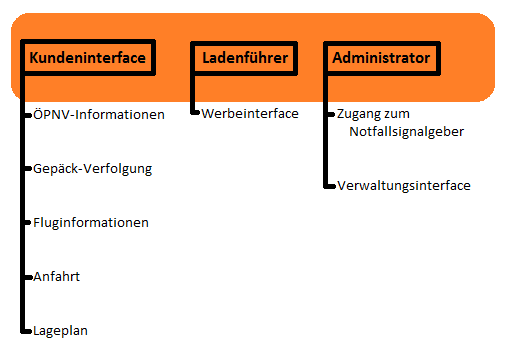
\includegraphics[scale=0.7]{psp_fach.png}
	\end{center}

}
%%-------------------------------------------------------
\frame{
	\frametitle{Phasen des Projektes}
	\begin{center}
		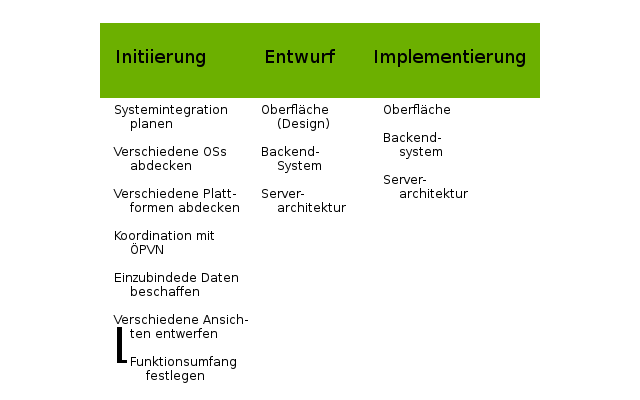
\includegraphics[scale=0.5]{psp_phasen.png}
	\end{center}


}
%%-------------------------------------------------------




\end{document}